\section{Traffic Management Optimization Using Multi-Objective Evolutionary Algorithms}

In this task, we have applyed a Multi-Objective Evolutionary Algorithm (MOEA) to optimize traffic management strategies for selected New York City (NYC) areas, in order to  minimize conflicting
objectives, Total Travel Time (TTT) and Fuel Consumption (FC), using real-world traffic data
from NYC Open Data. 
\newline
\newline
The traffic management strategy has involved controlling traffic signal timings (green, yellow, and red light durations), and setting speed limits on these segments. We have developed an MOEA that optimized these parameters to achieve the best trade-off between minimizing TTT and FC.

\subsection{Data Exploration, and Preprocessing}

In addition, we have used two datasets from the NYC Open Data portal:
1. NYC Traffic Volume Counts[1].
2. Traffic Speed Data[2].
\newline
\newline
The both datasets were collected from New York City Department of Transportation (NYC DOT). The first dataset uses Automated Traffic Recorders (ATR) to collect traffic sample volume counts at bridge crossings and roadways, and contains 31 columns[1], while the second dataset uses average speed of a vehicle traveled between end points, and contains 13 columns[2].
\newline
\newline
\begin{figure}[h]
    \centering
    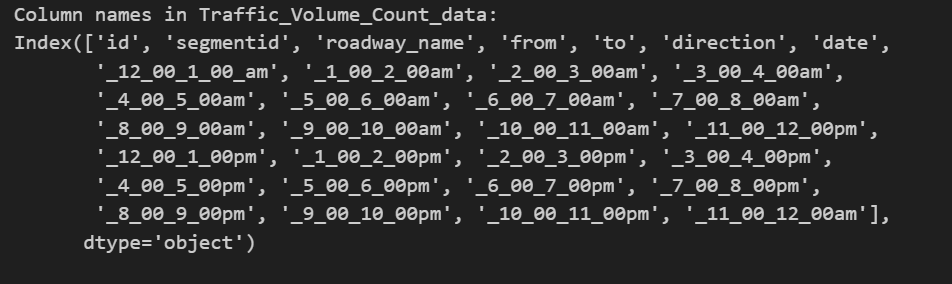
\includegraphics[width=1\linewidth]{figures/trafic_volume_count.PNG}
    \caption{Trafic Volume Count}
    \label{fig:Trafic Volume Count}
\end{figure}
\newline
\begin{figure}[h]
    \centering
    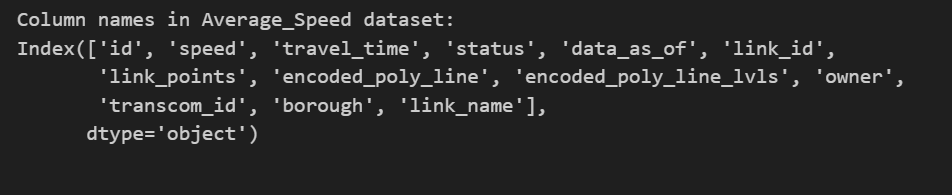
\includegraphics[width=1\linewidth]{figures/average_speed_dataset.PNG}
    \caption{Average Speed Of a Vehicle}
    \label{fig:Average Speed Of a Vehicle}
\end{figure}

We have focused on optimizing traffic management for the three road segments in New 
York City;  
1. 5th Ave between 42nd St and 47th St (Manhattan) 
2. Atlantic Ave between Flatbush Ave and Bedford Ave (Brooklyn).
3. Queens Blvd between Union Tpke and Yellowstone Blvd (Queens).
\newline
\begin{figure}[h]
    \centering
    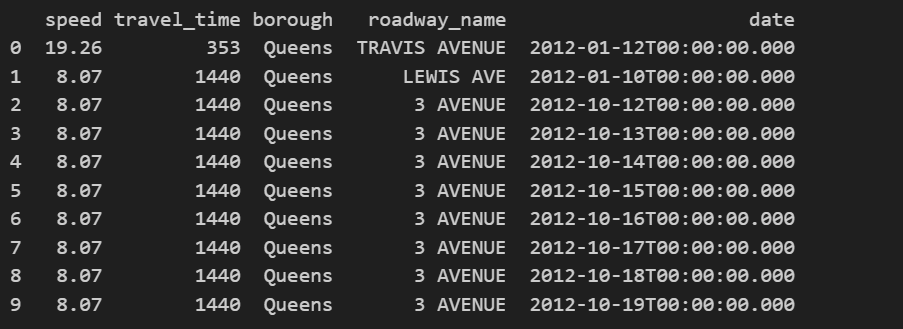
\includegraphics[width=1\linewidth]{figures/data_from_selected_area.PNG}
    \caption{Average Speed Of a Vehicle}
    \label{fig:Data From Selected Area}
\end{figure}
\newline
\newline
We have Identified and preprocess relevant data points, such as peak-hour traffic volumes, 
average speeds. The peak-hour trafik time has been calculated based on number of travel time in selected hours. The following figure showes the selected hours list.
\newline
\begin{figure}[h]
    \centering
    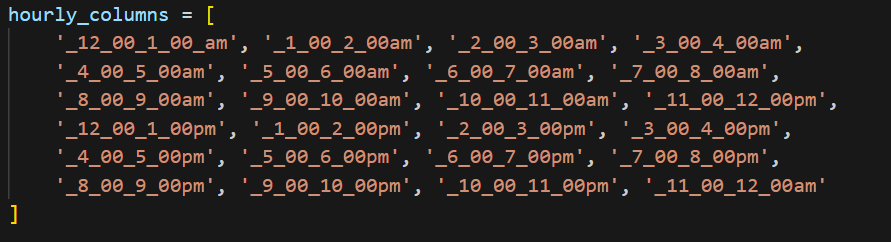
\includegraphics[width=1\linewidth]{figures/hours_list.PNG}
    \caption{Selected Hours List}
    \label{fig:The peak-hour Time}
\end{figure}
We have found that the Overall peak hour is between 5.00 Pm, and 6.00 PM, Overall volume: 14434156.0.
\newline
\begin{figure}[h]
    \centering
    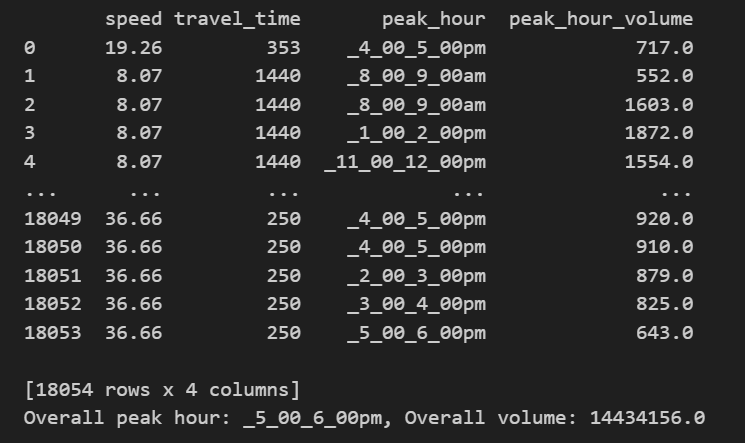
\includegraphics[width=1\linewidth]{figures/peak_huours_time.PNG}
    \caption{The peak-hour Time}
    \label{fig:The peak-hour Time}
\end{figure}
\newline




\subsection{Fuel Consumption Calculation}
Fuel consumption measures the amount of fuel a car consumes to go a specific distance[4]. 
We used the common fuel Consumption equation, defined as folowing:
\newline
\newline
Fuel Consumption = a × V + b × 1/v + c
\newline
Where: 
\newline
\newline
• V is the average speed (in mph). 
\newline
• a, b, and c are empirical const, which a indicating an increase in fuel consumption with speed, while b representing a decrease in fuel consumption as speed, and c represents the base fuel consumption, as very low-speed conditions.
\newline
\newline
Then, we have update the code to use the formula as following:
$Fuel Consumption=\sum_{i=1}^{n}  (volume_{i} \times (a×V_{i}+b×\frac{1}{v}+c)\times segment_Length_{i})$
\newline
\newline
where:
n is the number of time intervals. 
Volumei is the vehicle count in interval i from the Traffic 
Volume dataset. 
Vi is the average speed in interval i from the Traffic Speed dataset. 
Segment Lengthi is the length of the road segment.
\subsection{Formulate the Optimization Problem}
xxxxxx
\subsection{Implement the MOEA}
genetic algorithm
\subsection{Analysis and Results}

\begin{figure}[h]
    \centering
    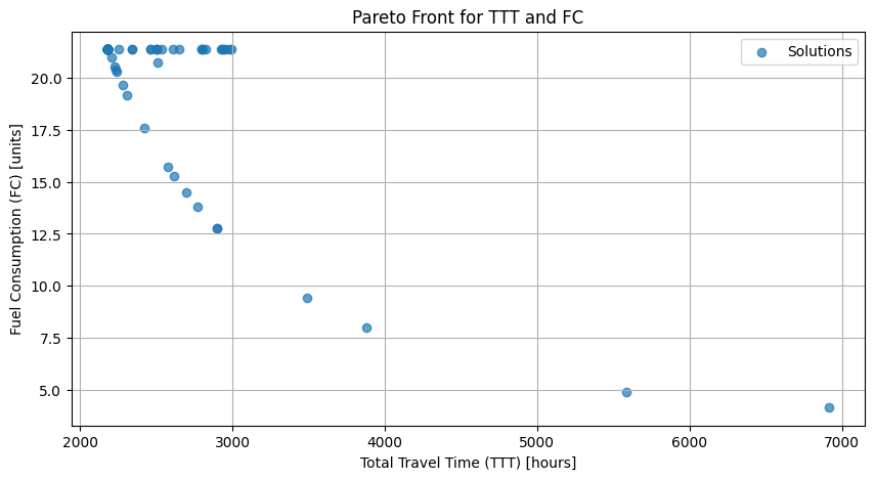
\includegraphics[width=0.7\textwidth]{figures/TTT.PNG}
    \caption{TTT}
    \label{fig:Total Travel Time}
\end{figure}

\begin{figure}[h]
    \centering
    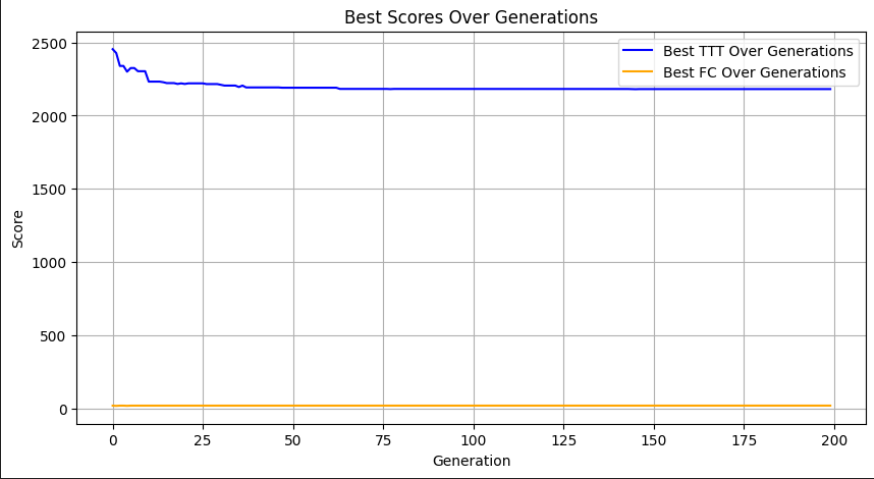
\includegraphics[width=0.7\textwidth]{figures/Best_score.PNG}
    \caption{The best score over generation}
    \label{fig:Best Score Over Generation} 
\end{figure}


